\documentclass{standalone}
\usepackage{tikz}
\usetikzlibrary{patterns, positioning}
\usepackage[sfdefault]{ClearSans} %% option 'sfdefault' activates Clear Sans as the default text font
\usepackage[T1]{fontenc}

\begin{document}
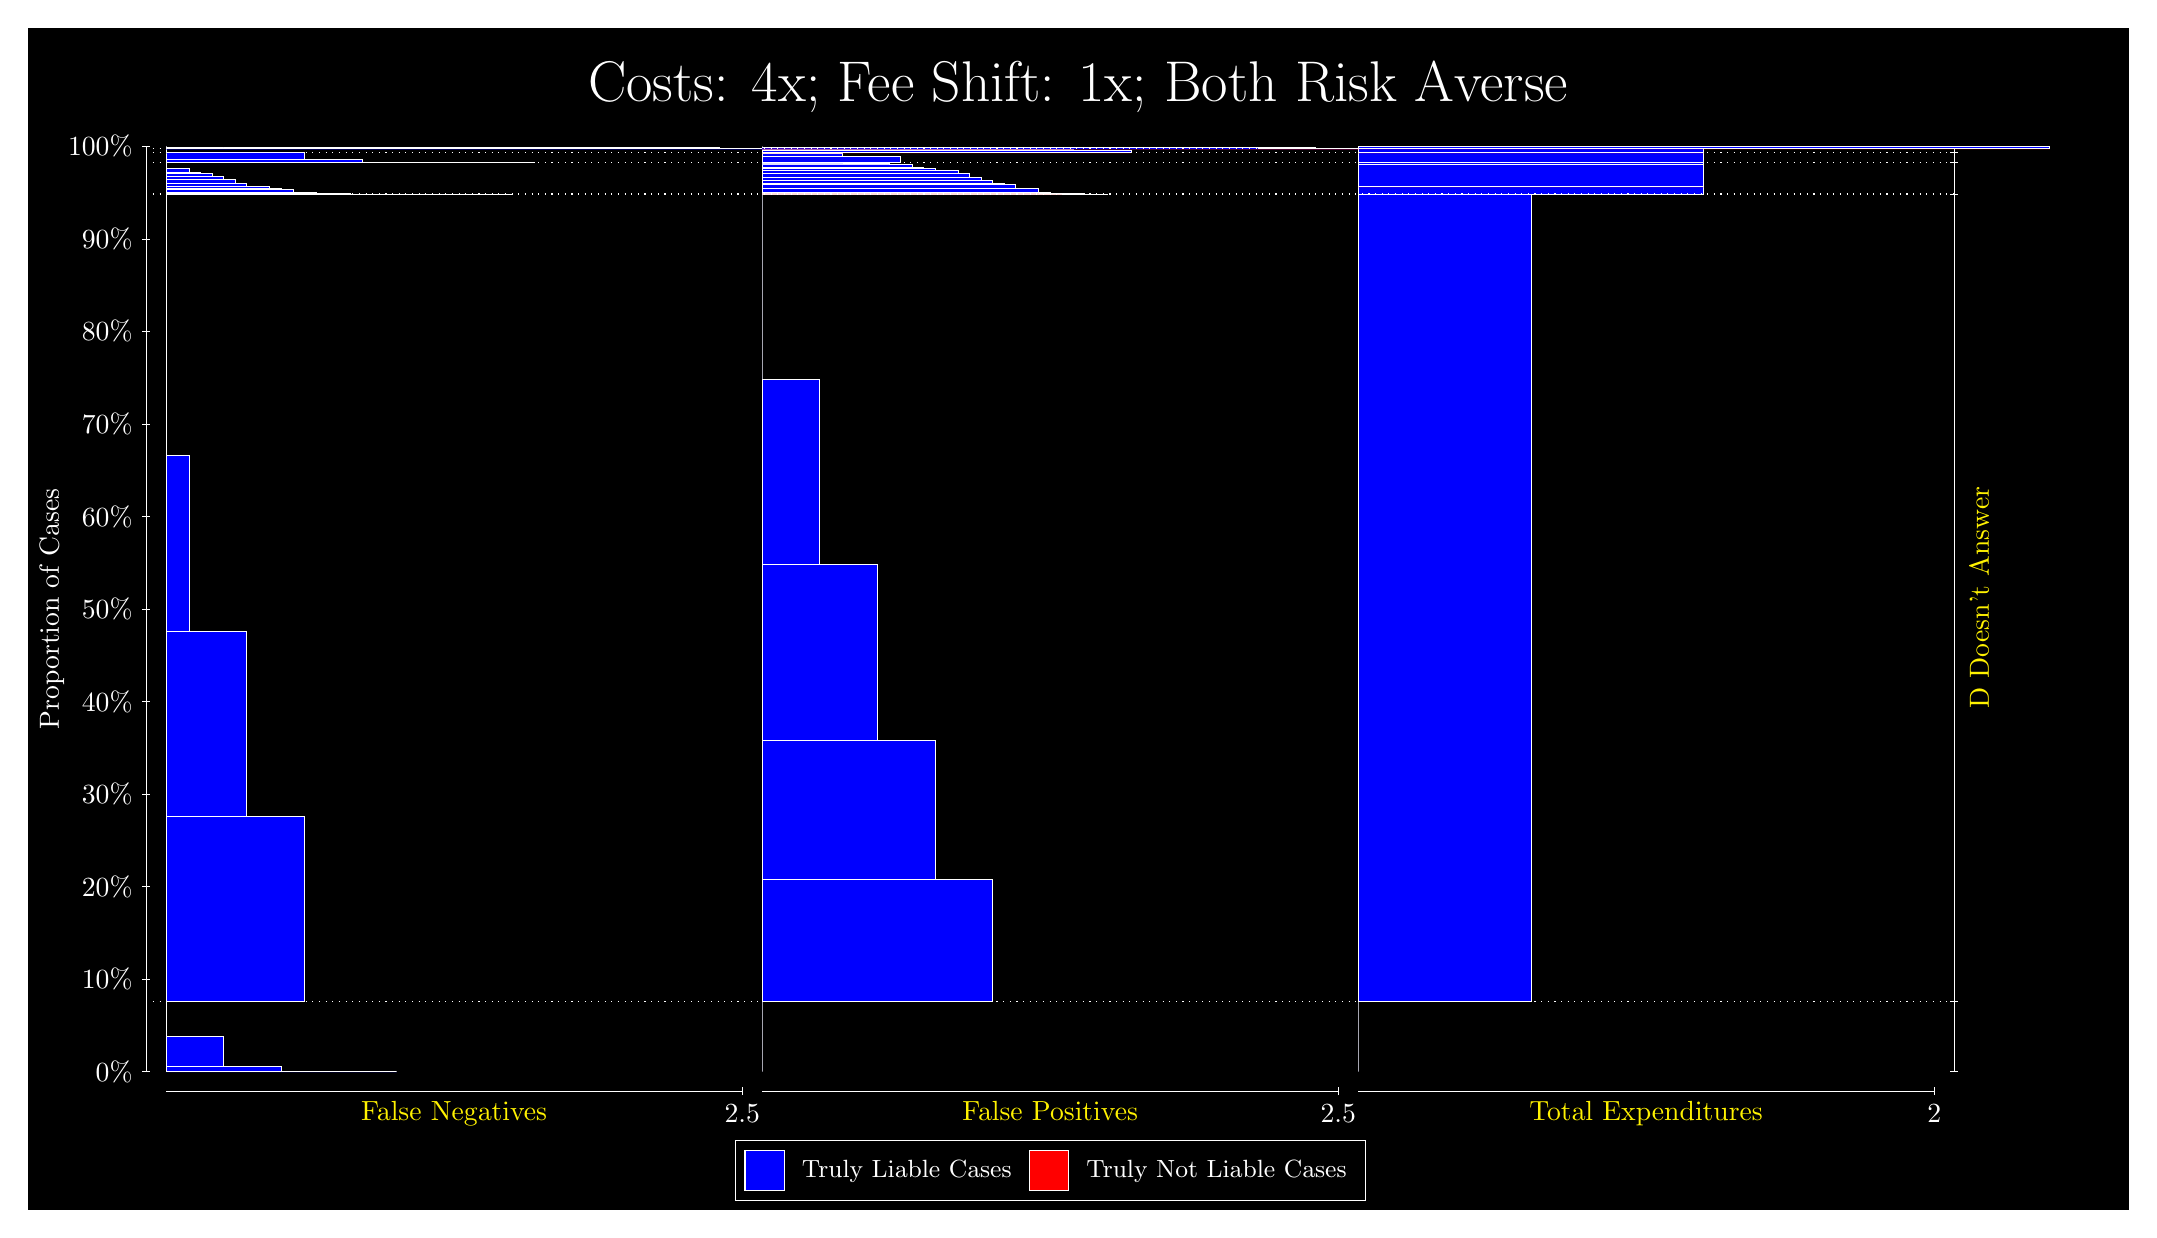
\begin{tikzpicture}
\draw[fill=black] (0,0) rectangle (26.667,15);
\draw[text=white] (0,13.5) rectangle (26.667,15) node[midway] {\huge Costs: 4x; Fee Shift: 1x; Both Risk Averse};
\draw[white, very thin] (1.5,1.75) -- (1.5,13.5);
\node[rotate=90, text=white, anchor=center] at (0.3, 7.625) {Proportion of Cases};
\draw[white, very thin] (1.45,1.75) -- (1.55,1.75);
\node[text=white, anchor=east] at (1.45, 1.75) {0\%};
\draw[white, very thin] (1.45,2.925) -- (1.55,2.925);
\node[text=white, anchor=east] at (1.45, 2.925) {10\%};
\draw[white, very thin] (1.45,4.1) -- (1.55,4.1);
\node[text=white, anchor=east] at (1.45, 4.1) {20\%};
\draw[white, very thin] (1.45,5.275) -- (1.55,5.275);
\node[text=white, anchor=east] at (1.45, 5.275) {30\%};
\draw[white, very thin] (1.45,6.45) -- (1.55,6.45);
\node[text=white, anchor=east] at (1.45, 6.45) {40\%};
\draw[white, very thin] (1.45,7.625) -- (1.55,7.625);
\node[text=white, anchor=east] at (1.45, 7.625) {50\%};
\draw[white, very thin] (1.45,8.8) -- (1.55,8.8);
\node[text=white, anchor=east] at (1.45, 8.8) {60\%};
\draw[white, very thin] (1.45,9.975) -- (1.55,9.975);
\node[text=white, anchor=east] at (1.45, 9.975) {70\%};
\draw[white, very thin] (1.45,11.15) -- (1.55,11.15);
\node[text=white, anchor=east] at (1.45, 11.15) {80\%};
\draw[white, very thin] (1.45,12.325) -- (1.55,12.325);
\node[text=white, anchor=east] at (1.45, 12.325) {90\%};
\draw[white, very thin] (1.45,13.5) -- (1.55,13.5);
\node[text=white, anchor=east] at (1.45, 13.5) {100\%};

\draw[white, very thin] (24.457,1.75) -- (24.457,13.5);
\draw[white, very thin] (24.407,1.75) -- (24.507,1.75);
\node[anchor=west] at (24.407, 1.75) {};
\draw[white, very thin] (24.407,2.6441) -- (24.507,2.6441);
\node[anchor=west] at (24.407, 2.6441) {};
\draw[white, very thin] (24.407,12.894) -- (24.507,12.894);
\node[anchor=west] at (24.407, 12.894) {};
\draw[white, very thin] (24.407,13.296) -- (24.507,13.296);
\node[anchor=west] at (24.407, 13.296) {};
\draw[white, very thin] (24.407,13.419) -- (24.507,13.419);
\node[anchor=west] at (24.407, 13.419) {};
\draw[white, very thin] (24.407,13.472) -- (24.507,13.472);
\node[anchor=west] at (24.407, 13.472) {};
\draw[white, very thin] (24.407,13.5) -- (24.507,13.5);
\node[anchor=west] at (24.407, 13.5) {};

\draw[white, very thin, fill=blue] (1.75,1.75) rectangle (4.6775,1.75);
\draw[white, very thin, fill=blue] (1.75,1.75) rectangle (3.9457,1.7506);
\draw[white, very thin, fill=blue] (1.75,1.7506) rectangle (3.2138,1.8216);
\draw[white, very thin, fill=blue] (1.75,1.8216) rectangle (2.4819,2.1977);
\draw[white, very thin, fill=red] (1.75,2.1977) rectangle (1.75,2.1977);
\draw[white, very thin, fill=blue] (1.75,2.1977) rectangle (1.75,2.6441);
\draw[white, very thin, fill=blue] (1.75,2.6441) rectangle (3.5065,4.994);
\draw[white, very thin, fill=blue] (1.75,4.994) rectangle (2.7746,7.3431);
\draw[white, very thin, fill=blue] (1.75,7.3431) rectangle (2.0428,9.582);
\draw[white, very thin, fill=red] (1.75,9.582) rectangle (1.75,9.582);
\draw[white, very thin, fill=blue] (1.75,9.582) rectangle (1.75,12.894);
\draw[white, very thin, fill=blue] (1.75,12.894) rectangle (6.1413,12.894);
\draw[white, very thin, fill=blue] (1.75,12.894) rectangle (5.8486,12.894);
\draw[white, very thin, fill=blue] (1.75,12.894) rectangle (5.5558,12.894);
\draw[white, very thin, fill=blue] (1.75,12.894) rectangle (5.4094,12.894);
\draw[white, very thin, fill=blue] (1.75,12.894) rectangle (5.2631,12.894);
\draw[white, very thin, fill=blue] (1.75,12.894) rectangle (5.1167,12.894);
\draw[white, very thin, fill=blue] (1.75,12.894) rectangle (4.9703,12.894);
\draw[white, very thin, fill=blue] (1.75,12.894) rectangle (4.8239,12.894);
\draw[white, very thin, fill=blue] (1.75,12.894) rectangle (4.6775,12.895);
\draw[white, very thin, fill=blue] (1.75,12.895) rectangle (4.5312,12.895);
\draw[white, very thin, fill=blue] (1.75,12.895) rectangle (4.3848,12.895);
\draw[white, very thin, fill=blue] (1.75,12.895) rectangle (4.3848,12.896);
\draw[white, very thin, fill=blue] (1.75,12.896) rectangle (4.2384,12.896);
\draw[white, very thin, fill=blue] (1.75,12.896) rectangle (4.092,12.901);
\draw[white, very thin, fill=blue] (1.75,12.901) rectangle (4.092,12.901);
\draw[white, very thin, fill=blue] (1.75,12.901) rectangle (3.9457,12.905);
\draw[white, very thin, fill=blue] (1.75,12.905) rectangle (3.7993,12.909);
\draw[white, very thin, fill=blue] (1.75,12.909) rectangle (3.6529,12.909);
\draw[white, very thin, fill=blue] (1.75,12.909) rectangle (3.6529,12.913);
\draw[white, very thin, fill=blue] (1.75,12.913) rectangle (3.5065,12.919);
\draw[white, very thin, fill=blue] (1.75,12.919) rectangle (3.3602,12.953);
\draw[white, very thin, fill=blue] (1.75,12.953) rectangle (3.3602,12.953);
\draw[white, very thin, fill=blue] (1.75,12.953) rectangle (3.2138,12.963);
\draw[white, very thin, fill=blue] (1.75,12.963) rectangle (3.0674,12.965);
\draw[white, very thin, fill=blue] (1.75,12.965) rectangle (3.0674,12.99);
\draw[white, very thin, fill=blue] (1.75,12.99) rectangle (2.921,12.992);
\draw[white, very thin, fill=blue] (1.75,12.992) rectangle (2.921,12.995);
\draw[white, very thin, fill=blue] (1.75,12.995) rectangle (2.7746,13.028);
\draw[white, very thin, fill=blue] (1.75,13.028) rectangle (2.6283,13.084);
\draw[white, very thin, fill=blue] (1.75,13.084) rectangle (2.6283,13.085);
\draw[white, very thin, fill=blue] (1.75,13.085) rectangle (2.4819,13.115);
\draw[white, very thin, fill=blue] (1.75,13.115) rectangle (2.3355,13.118);
\draw[white, very thin, fill=blue] (1.75,13.118) rectangle (2.3355,13.161);
\draw[white, very thin, fill=blue] (1.75,13.161) rectangle (2.1891,13.169);
\draw[white, very thin, fill=blue] (1.75,13.169) rectangle (2.0428,13.223);
\draw[white, very thin, fill=blue] (1.75,13.223) rectangle (1.8964,13.225);
\draw[white, very thin, fill=red] (1.75,13.225) rectangle (1.75,13.225);
\draw[white, very thin, fill=blue] (1.75,13.225) rectangle (1.75,13.296);
\draw[white, very thin, fill=blue] (1.75,13.296) rectangle (6.4341,13.296);
\draw[white, very thin, fill=blue] (1.75,13.296) rectangle (5.7022,13.296);
\draw[white, very thin, fill=blue] (1.75,13.296) rectangle (4.9703,13.301);
\draw[white, very thin, fill=blue] (1.75,13.301) rectangle (4.2384,13.34);
\draw[white, very thin, fill=blue] (1.75,13.34) rectangle (3.5065,13.419);
\draw[white, very thin, fill=red] (1.75,13.419) rectangle (1.75,13.419);
\draw[white, very thin, fill=blue] (1.75,13.419) rectangle (3.5065,13.419);
\draw[white, very thin, fill=blue] (1.75,13.419) rectangle (2.7746,13.419);
\draw[white, very thin, fill=blue] (1.75,13.419) rectangle (2.0428,13.425);
\draw[white, very thin, fill=red] (1.75,13.425) rectangle (1.75,13.425);
\draw[white, very thin, fill=blue] (1.75,13.425) rectangle (1.75,13.472);
\draw[white, very thin, fill=blue] (1.75,13.472) rectangle (11.704,13.472);
\draw[white, very thin, fill=blue] (1.75,13.472) rectangle (10.972,13.472);
\draw[white, very thin, fill=blue] (1.75,13.472) rectangle (10.24,13.472);
\draw[white, very thin, fill=blue] (1.75,13.472) rectangle (9.508,13.475);
\draw[white, very thin, fill=blue] (1.75,13.475) rectangle (8.7761,13.487);
\draw[white, very thin, fill=blue] (1.75,13.487) rectangle (8.0442,13.489);
\draw[white, very thin, fill=blue] (1.75,13.489) rectangle (7.3123,13.489);
\draw[white, very thin, fill=blue] (1.75,13.489) rectangle (3.9457,13.489);
\draw[white, very thin, fill=blue] (1.75,13.489) rectangle (3.2138,13.489);
\draw[white, very thin, fill=blue] (1.75,13.489) rectangle (2.4819,13.489);
\draw[white, very thin, fill=red] (1.75,13.489) rectangle (1.75,13.489);
\draw[white, very thin, fill=blue] (1.75,13.489) rectangle (1.75,13.5);
\draw[white, very thin, fill=red] (9.3189,1.75) rectangle (9.3189,1.75);
\draw[white, very thin, fill=blue] (9.3189,1.75) rectangle (9.3189,2.6441);
\draw[white, very thin, fill=red] (9.3189,2.6441) rectangle (12.246,2.6441);
\draw[white, very thin, fill=blue] (9.3189,2.6441) rectangle (12.246,4.1938);
\draw[white, very thin, fill=blue] (9.3189,4.1938) rectangle (11.515,5.9556);
\draw[white, very thin, fill=blue] (9.3189,5.9556) rectangle (10.783,8.1946);
\draw[white, very thin, fill=blue] (9.3189,8.1946) rectangle (10.051,10.544);
\draw[white, very thin, fill=blue] (9.3189,10.544) rectangle (9.3189,12.894);
\draw[white, very thin, fill=red] (9.3189,12.894) rectangle (13.71,12.894);
\draw[white, very thin, fill=blue] (9.3189,12.894) rectangle (13.71,12.896);
\draw[white, very thin, fill=red] (9.3189,12.896) rectangle (13.417,12.896);
\draw[white, very thin, fill=blue] (9.3189,12.896) rectangle (13.417,12.898);
\draw[white, very thin, fill=red] (9.3189,12.898) rectangle (13.125,12.898);
\draw[white, very thin, fill=blue] (9.3189,12.898) rectangle (13.125,12.91);
\draw[white, very thin, fill=blue] (9.3189,12.91) rectangle (12.978,12.912);
\draw[white, very thin, fill=red] (9.3189,12.912) rectangle (12.832,12.912);
\draw[white, very thin, fill=blue] (9.3189,12.912) rectangle (12.832,12.965);
\draw[white, very thin, fill=blue] (9.3189,12.965) rectangle (12.686,12.966);
\draw[white, very thin, fill=red] (9.3189,12.966) rectangle (12.539,12.966);
\draw[white, very thin, fill=blue] (9.3189,12.966) rectangle (12.539,13.021);
\draw[white, very thin, fill=blue] (9.3189,13.021) rectangle (12.393,13.029);
\draw[white, very thin, fill=red] (9.3189,13.029) rectangle (12.246,13.029);
\draw[white, very thin, fill=blue] (9.3189,13.029) rectangle (12.246,13.075);
\draw[white, very thin, fill=blue] (9.3189,13.075) rectangle (12.1,13.105);
\draw[white, very thin, fill=red] (9.3189,13.105) rectangle (11.954,13.105);
\draw[white, very thin, fill=blue] (9.3189,13.105) rectangle (11.954,13.162);
\draw[white, very thin, fill=blue] (9.3189,13.162) rectangle (11.807,13.195);
\draw[white, very thin, fill=red] (9.3189,13.195) rectangle (11.661,13.195);
\draw[white, very thin, fill=blue] (9.3189,13.195) rectangle (11.661,13.198);
\draw[white, very thin, fill=blue] (9.3189,13.198) rectangle (11.661,13.2);
\draw[white, very thin, fill=blue] (9.3189,13.2) rectangle (11.515,13.227);
\draw[white, very thin, fill=red] (9.3189,13.227) rectangle (11.368,13.227);
\draw[white, very thin, fill=blue] (9.3189,13.227) rectangle (11.368,13.236);
\draw[white, very thin, fill=blue] (9.3189,13.236) rectangle (11.222,13.271);
\draw[white, very thin, fill=blue] (9.3189,13.271) rectangle (11.075,13.277);
\draw[white, very thin, fill=blue] (9.3189,13.277) rectangle (10.929,13.281);
\draw[white, very thin, fill=blue] (9.3189,13.281) rectangle (10.929,13.281);
\draw[white, very thin, fill=blue] (9.3189,13.281) rectangle (10.783,13.285);
\draw[white, very thin, fill=blue] (9.3189,13.285) rectangle (10.636,13.288);
\draw[white, very thin, fill=blue] (9.3189,13.288) rectangle (10.49,13.294);
\draw[white, very thin, fill=blue] (9.3189,13.294) rectangle (10.344,13.294);
\draw[white, very thin, fill=blue] (9.3189,13.294) rectangle (10.197,13.295);
\draw[white, very thin, fill=blue] (9.3189,13.295) rectangle (10.197,13.295);
\draw[white, very thin, fill=blue] (9.3189,13.295) rectangle (10.051,13.295);
\draw[white, very thin, fill=blue] (9.3189,13.295) rectangle (9.9044,13.296);
\draw[white, very thin, fill=blue] (9.3189,13.296) rectangle (9.758,13.296);
\draw[white, very thin, fill=blue] (9.3189,13.296) rectangle (9.6116,13.296);
\draw[white, very thin, fill=blue] (9.3189,13.296) rectangle (9.4652,13.296);
\draw[white, very thin, fill=blue] (9.3189,13.296) rectangle (9.3189,13.296);
\draw[white, very thin, fill=red] (9.3189,13.296) rectangle (11.075,13.296);
\draw[white, very thin, fill=blue] (9.3189,13.296) rectangle (11.075,13.375);
\draw[white, very thin, fill=blue] (9.3189,13.375) rectangle (10.344,13.414);
\draw[white, very thin, fill=blue] (9.3189,13.414) rectangle (9.6116,13.419);
\draw[white, very thin, fill=blue] (9.3189,13.419) rectangle (9.3189,13.419);
\draw[white, very thin, fill=red] (9.3189,13.419) rectangle (14.003,13.419);
\draw[white, very thin, fill=blue] (9.3189,13.419) rectangle (14.003,13.445);
\draw[white, very thin, fill=blue] (9.3189,13.445) rectangle (13.271,13.467);
\draw[white, very thin, fill=blue] (9.3189,13.467) rectangle (12.539,13.472);
\draw[white, very thin, fill=blue] (9.3189,13.472) rectangle (11.807,13.472);
\draw[white, very thin, fill=blue] (9.3189,13.472) rectangle (11.075,13.472);
\draw[white, very thin, fill=red] (9.3189,13.472) rectangle (19.273,13.472);
\draw[white, very thin, fill=blue] (9.3189,13.472) rectangle (19.273,13.472);
\draw[white, very thin, fill=red] (9.3189,13.472) rectangle (18.541,13.472);
\draw[white, very thin, fill=blue] (9.3189,13.472) rectangle (18.541,13.472);
\draw[white, very thin, fill=red] (9.3189,13.472) rectangle (17.809,13.472);
\draw[white, very thin, fill=blue] (9.3189,13.472) rectangle (17.809,13.473);
\draw[white, very thin, fill=red] (9.3189,13.473) rectangle (17.077,13.473);
\draw[white, very thin, fill=blue] (9.3189,13.473) rectangle (17.077,13.479);
\draw[white, very thin, fill=blue] (9.3189,13.479) rectangle (16.345,13.483);
\draw[white, very thin, fill=blue] (9.3189,13.483) rectangle (15.613,13.484);
\draw[white, very thin, fill=blue] (9.3189,13.484) rectangle (14.881,13.484);
\draw[white, very thin, fill=blue] (9.3189,13.484) rectangle (14.149,13.484);
\draw[white, very thin, fill=red] (9.3189,13.484) rectangle (10.783,13.484);
\draw[white, very thin, fill=blue] (9.3189,13.484) rectangle (10.783,13.484);
\draw[white, very thin, fill=red] (9.3189,13.484) rectangle (10.051,13.484);
\draw[white, very thin, fill=blue] (9.3189,13.484) rectangle (10.051,13.486);
\draw[white, very thin, fill=red] (9.3189,13.486) rectangle (9.3189,13.486);
\draw[white, very thin, fill=blue] (9.3189,13.486) rectangle (9.3189,13.5);
\draw[white, very thin, fill=red] (16.888,1.75) rectangle (16.888,1.75);
\draw[white, very thin, fill=blue] (16.888,1.75) rectangle (16.888,2.6441);
\draw[white, very thin, fill=red] (16.888,2.6441) rectangle (19.083,2.6441);
\draw[white, very thin, fill=blue] (16.888,2.6441) rectangle (19.083,12.894);
\draw[white, very thin, fill=red] (16.888,12.894) rectangle (21.279,12.894);
\draw[white, very thin, fill=blue] (16.888,12.894) rectangle (21.279,12.987);
\draw[white, very thin, fill=red] (16.888,12.987) rectangle (21.279,12.987);
\draw[white, very thin, fill=blue] (16.888,12.987) rectangle (21.279,13.27);
\draw[white, very thin, fill=red] (16.888,13.27) rectangle (21.279,13.27);
\draw[white, very thin, fill=blue] (16.888,13.27) rectangle (21.279,13.296);
\draw[white, very thin, fill=red] (16.888,13.296) rectangle (21.279,13.296);
\draw[white, very thin, fill=blue] (16.888,13.296) rectangle (21.279,13.419);
\draw[white, very thin, fill=red] (16.888,13.419) rectangle (21.279,13.419);
\draw[white, very thin, fill=blue] (16.888,13.419) rectangle (21.279,13.472);
\draw[white, very thin, fill=red] (16.888,13.472) rectangle (25.67,13.472);
\draw[white, very thin, fill=blue] (16.888,13.472) rectangle (25.67,13.5);
\draw[white, dotted] (1.5,2.6441) -- (24.457,2.6441);
\draw[white, dotted] (1.5,12.894) -- (24.457,12.894);
\draw[white, dotted] (1.5,13.296) -- (24.457,13.296);
\draw[white, dotted] (1.5,13.419) -- (24.457,13.419);
\draw[white, dotted] (1.5,13.472) -- (24.457,13.472);
\draw[white, very thin] (1.75,1.5) -- (9.0689,1.5);
\node[text=yellow, anchor=north] at (5.4094, 1.5) {False Negatives};
\draw[white, very thin] (9.0689,1.45) -- (9.0689,1.55);
\node[text=white, anchor=north] at (9.0689, 1.45) {2.5};

\draw[white, very thin] (9.3189,1.5) -- (16.638,1.5);
\node[text=yellow, anchor=north] at (12.978, 1.5) {False Positives};
\draw[white, very thin] (16.638,1.45) -- (16.638,1.55);
\node[text=white, anchor=north] at (16.638, 1.45) {2.5};

\draw[white, very thin] (16.888,1.5) -- (24.207,1.5);
\node[text=yellow, anchor=north] at (20.547, 1.5) {Total Expenditures};
\draw[white, very thin] (24.207,1.45) -- (24.207,1.55);
\node[text=white, anchor=north] at (24.207, 1.45) {2};


\node[text=yellow, centered, rotate=90] at (24.777, 7.7688) {D Doesn't Answer};





\draw (12.978300999999998,1.5) node[draw=none] (baseCoordinate) {};
\begin{scope}[align=center]
        \matrix[scale=0.5, draw=white, below=0.5cm of baseCoordinate, nodes={draw}, column sep=0.1cm]{
            \node[rectangle, draw, minimum width=0.5cm, minimum height=0.5cm, fill=blue] {}; &
            \node[draw=none, font=\small, text=white] (B) {Truly Liable Cases}; &
            \node[rectangle, draw, minimum width=0.5cm, minimum height=0.5cm, fill=red] {}; &
            \node[draw=none, font=\small, text=white] (B) {Truly Not Liable Cases}; \\
            };
\end{scope}

\end{tikzpicture}
\end{document}